% !TEX program = xelatex
% Generated by scripts/build_report.py from real saved analysis outputs.
\documentclass[UTF8,fontset=none,zihao=-4]{ctexart}
% Locally use the system TrueType font whose Chinese rendering was verified.
% On systems without it (including typical Overleaf projects), use Fandol.
\IfFontExistsTF{Arial Unicode MS}{
  \setCJKmainfont[AutoFakeBold=2]{Arial Unicode MS}
  \setCJKsansfont[AutoFakeBold=2]{Arial Unicode MS}
  \setCJKmonofont{Arial Unicode MS}
  \setCJKfamilyfont{hei}[AutoFakeBold=2]{Arial Unicode MS}
  \setCJKfamilyfont{song}[AutoFakeBold=2]{Arial Unicode MS}
}{
  \setCJKmainfont[BoldFont=FandolSong-Bold.otf,ItalicFont=FandolKai-Regular.otf]{FandolSong-Regular.otf}
  \setCJKsansfont[BoldFont=FandolHei-Bold.otf]{FandolHei-Regular.otf}
  \setCJKmonofont{FandolFang-Regular.otf}
  \setCJKfamilyfont{hei}[BoldFont=FandolHei-Bold.otf]{FandolHei-Regular.otf}
  \setCJKfamilyfont{song}[BoldFont=FandolSong-Bold.otf]{FandolSong-Regular.otf}
}
\providecommand{\heiti}{\CJKfamily{hei}}
\providecommand{\songti}{\CJKfamily{song}}
\usepackage[a4paper,left=24mm,right=24mm,top=23mm,bottom=24mm]{geometry}
\usepackage{amsmath,amssymb,booktabs,array,longtable,graphicx,float,placeins,pdflscape}
\usepackage{xurl}
\usepackage{xcolor,hyperref,fancyhdr,enumitem,caption,microtype,seqsplit}
\hypersetup{colorlinks=true,linkcolor=blue!45!black,citecolor=blue!45!black,urlcolor=blue!45!black,breaklinks=true}
\usepackage[numbers,sort&compress]{natbib}
\setlength{\parindent}{2em}
\setlength{\parskip}{3pt}
\linespread{1.25}
\setlist{nosep,leftmargin=2em}
\captionsetup{font=small,labelfont=bf,labelsep=quad}
\pagestyle{fancy}\fancyhf{}
\fancyhead[L]{\small Python 课程项目：WDBC 特征减量}
\fancyfoot[C]{\small \thepage}
\setlength{\headheight}{16pt}
\renewcommand{\headrulewidth}{0.3pt}
\graphicspath{{figures/}}
% Generated from saved analysis and the applicable profile; approved public author name only.
\newcommand{\AuthorName}{潘冠宇}
\newcommand{\StudentID}{}
\newcommand{\Institution}{}
\newcommand{\TotalN}{569}
\newcommand{\BenignN}{357}
\newcommand{\MalignantN}{212}
\newcommand{\DevelopmentN}{455}
\newcommand{\TestN}{114}
\newcommand{\DevelopmentB}{285}
\newcommand{\DevelopmentM}{170}
\newcommand{\TestB}{72}
\newcommand{\TestM}{42}
\newcommand{\BootstrapN}{1000}
\newcommand{\DefaultModel}{LR30}
\newcommand{\HomepageURL}{\url{https://aapan818-web.github.io/wdbc-feature-reduction/}}
\newcommand{\ProjectURL}{\url{https://aapan818-web.github.io/wdbc-feature-reduction/project/}}
\newcommand{\RepositoryURL}{\url{https://github.com/aapan818-web/wdbc-feature-reduction}}
\newcommand{\LRFullAUC}{0.9960}
\newcommand{\LRFullCVAUC}{0.9958}
\newcommand{\LRFullFN}{3}
\newcommand{\LRFullFP}{1}
\newcommand{\LRFullSensitivity}{0.929}
\newcommand{\LRTenAUC}{0.9974}
\newcommand{\LRTenCVAUC}{0.9851}
\newcommand{\LRTenFN}{4}
\newcommand{\LRTenFP}{1}
\newcommand{\LRTenSensitivity}{0.905}
\newcommand{\LRFiveAUC}{0.9957}
\newcommand{\LRFiveCVAUC}{0.9850}
\newcommand{\LRFiveFN}{3}
\newcommand{\LRFiveFP}{1}
\newcommand{\LRFiveSensitivity}{0.929}
\newcommand{\RFFullAUC}{0.9940}
\newcommand{\RFFullCVAUC}{0.9870}
\newcommand{\RFFullFN}{4}
\newcommand{\RFFullFP}{0}
\newcommand{\RFFullSensitivity}{0.905}

\title{\vspace{-1em}\heiti 乳腺肿块良恶性分类中的特征减量\\[0.6em]\large 5、10、30 个细胞核特征下的分类表现与解释}
\author{\AuthorName}
\date{2026 年 11 月 13 日}
\begin{document}
\maketitle
\thispagestyle{empty}
\begin{abstract}
\noindent\textbf{目的：}在固定模型设置和验证流程下，比较 WDBC 数据中使用全部 30 个特征与保留 10 个或 5 个特征的逻辑回归分类表现，分析特征冗余、筛选稳定性与误判。\textbf{方法：}读取课程提供的公开 WDBC 数据，明确恶性为正类；按类别分层划分开发集与测试集，在开发集内采用共用五折交叉验证。标准化及单变量特征筛选均放入训练管道，另设置无信息基线及随机森林参照。对开发集中三项预设变量进行分布比较、Holm 校正和效应量估计；在测试集报告 AUC、分类指标及分层成对 bootstrap 差值区间。\textbf{结果：}共纳入 \TotalN{} 条记录，开发集 \DevelopmentN{} 条、测试集 \TestN{} 条。LR30、LR10、LR5 的测试 AUC 分别为 \LRFullAUC{}、\LRTenAUC{} 和 \LRFiveAUC{}，对应漏判恶性样本 \LRFullFN{}、\LRTenFN{} 和 \LRFiveFN{} 条。\textbf{结论：}本实验给出了同一数据与固定设置下特征减量的实际表现及不确定性。模型简化的判断须同时考虑排序能力、错误计数和选择稳定性；分数接近不构成等效证明，也不能据此宣称减少临床检查或降低费用。
\end{abstract}
\noindent\textbf{关键词：}WDBC；特征选择；逻辑回归；交叉验证；分类评价；可复现分析

\vspace{0.6em}
\noindent\fcolorbox{blue!30!black}{blue!3}{\parbox{0.94\linewidth}{\small 本报告已由真实分析结果生成；作者仍需逐项理解并核对数据、方法、数字、图表和引用。当前提交前待办：个人主页资料由作者后续提供，公开URL待填写并核验。}}
\newpage

\section{背景与研究问题}
WDBC 是用于乳腺肿块良恶性分类的公开数据集。输入为乳腺肿块细针穿刺数字图像中提取的细胞核数值特征，目标为已有的良性或恶性标签\cite{uci}. 同一基础特征具有 mean、standard error（SE）和 worst 三类摘要，因此多个变量可能携带相关信息。增加输入数量可能提高表达能力，也可能引入冗余；实际影响需要在一致的验证条件下比较。

本项目回答：在使用相同逻辑回归设置时，将输入从 30 个减为 10 个或 5 个，分类表现、入选特征和错误类型如何变化？主要比较为测试 AUC 差值 $\mathrm{AUC}_{5}-\mathrm{AUC}_{30}$ 和 $\mathrm{AUC}_{10}-\mathrm{AUC}_{30}$。无信息基线帮助理解仅利用类别比例的表现，随机森林作为预设非线性参照。模型设置在评价前固定，不通过反复查看测试分数挑选参数。

本研究属于公开既有数据的回顾性方法比较，不采集新患者，也不预测未来发病。减少数值输入并不等于减少检查次数：这些特征来自同类图像，而非 30 项独立临床检查。本作业不提出临床安全性、成本效益或可部署诊断工具的结论。

\section{数据与方法}
\subsection{来源、字段与读取}
数据来自课程提供的 \texttt{wdbc.csv} 及其配套 \texttt{wdbc.names}，原始来源为 UCI\cite{uci}. CSV 无表头，读取时使用 \texttt{header=None}，再赋予固定的 32 个字段名，避免将第一条样本当成列名。ID 用于追踪记录，不作为预测输入；标签映射为 B=0、M=1。

30 个输入由半径、纹理、周长、面积、平滑度、紧致度、凹度、凹点、对称性及分形维数各自的三种摘要构成。数据按 10 个 mean、10 个 SE、10 个 worst 排列；worst 在说明文件中指三个最大值的均值，不能解释为病情分级。本项目沿用源数据数值尺度，不为缺少明示单位的字段补造单位。

\subsection{数据质量与预处理}
分析脚本检查行列数、标签范围、数值类型、缺失值、非有限值、重复 ID 和重复特征行。原始文件保持不变，工作数据和划分清单另行保存；核查结果见附录。数据处理不因某条记录降低预测分数而删除它。模型输入移除 ID 与诊断标签，防止标识或答案进入特征矩阵。

逻辑回归使用训练内标准化：$z=(x-\mu_{\mathrm{train}})/\sigma_{\mathrm{train}}$。验证或测试数据只沿用已拟合的参数。LR10 与 LR5 使用 \texttt{SelectKBest(f\_classif)} 保留指定数量的原始变量。该方法逐变量衡量组间区分程度，不穷举组合，也不保证去除相关变量或得到全局最优特征集。标准化、筛选和分类器组成 \texttt{Pipeline}，每个交叉验证折重新拟合，以免验证信息提前进入处理规则\cite{sklearnpitfalls,selectkbest}。

\subsection{数据划分与模型设置}
按类别分层，以随机种子 42 将 80\% 数据分配至开发集、20\% 分配至测试集。开发集采用五折 \texttt{StratifiedKFold}，打乱且随机种子固定为 42；全部模型共用相同折。数据划分构成如下。
\begin{center}
\small
\setlength{\tabcolsep}{5pt}
\renewcommand{\arraystretch}{1.25}
\begin{tabular}{lrrr}
\toprule
数据集 & 总数 & 良性 B & 恶性 M \tabularnewline
\midrule
全部记录 & 569 & 357 & 212 \tabularnewline
开发集 & 455 & 285 & 170 \tabularnewline
最终测试集 & 114 & 72 & 42 \tabularnewline
\bottomrule
\end{tabular}
\end{center}
{\footnotesize 恶性 M 编码为 1，是全部分类指标的正类；良性 B 编码为 0。}


预设模型为：DUMMY 使用 \texttt{strategy=prior}；LR30、LR10、LR5 使用相同 L2 正则化逻辑回归，$C=1$、\texttt{solver=lbfgs}、\texttt{max\_iter=2000}，仅保留特征数量不同；RF30 使用全部 30 个特征，200 棵树、最大深度 4、叶节点最少 5 个样本、随机种子 42。随机森林不要求进行相同的标准化处理。实际参数与软件版本随输出记录；新版 scikit-learn 用 \texttt{l1\_ratio=0} 表达此处预设的 L2 惩罚。

展示默认模型只在三个逻辑回归候选中，根据开发集平均 CV AUC 确定，精确同分时优先较少特征；本次为 \DefaultModel{}。这不是按测试成绩选出的“最佳模型”。全部预设模型在完整开发集上重拟合，再统一评价同一测试集；分类阈值均固定为 0.5，不称为临床最佳阈值。

\subsection{描述统计与三项预设组间比较}
涉及标签的分布探索、相关结构及组间比较限制在开发集。预先选择 \texttt{mean\_radius}、\texttt{mean\_texture}、\texttt{mean\_smoothness}，分别体现大小、纹理和局部边缘变化；报告两组中位数、第一及第三四分位数。对三项变量实施双侧 Mann--Whitney U 检验，使用 Holm 方法校正三项 P 值。该检验针对两组分布，不能在缺乏额外条件时一概称为中位数检验\cite{mannwhitney}。

恶性组作为 U 统计量第一组，秩二列相关定义为
\begin{equation}
r_{rb}=\frac{2U_M}{n_M n_B}-1.
\end{equation}
正值表示恶性组取值通常较高；在良性与恶性组内分别进行 \BootstrapN{} 次有放回重采样，以百分位法得到 95\% 区间，随机种子为 20261113。这些统计检验用于描述数据，不用于生成最终模型特征名单。30 个特征的 Spearman 相关热图用于探索信息冗余，不对所有相关系数逐个进行显著性检验。

补充诊断记录组内 Shapiro--Wilk、以中位数为中心的 Levene 检验和 1.5 倍四分位距筛查，结果保存在 \texttt{outputs/diagnostics.json}；这些数值筛查不用于事后切换检验或删除样本。分析按记录独立处理，唯一 ID 本身不能充分证明原始采样的独立性。

\subsection{评价、不确定性与解释}
主要指标为 ROC-AUC，以恶性类别连续分数计算。另报告灵敏度 $TP/(TP+FN)$、特异度 $TN/(TN+FP)$、精确率 $TP/(TP+FP)$、F1 和准确率，并列出混淆计数。无阳性预测时，精确率没有定义，不用一个看似有效的零掩盖这一情形。CV 的均值与标准差描述五折间的波动，标准差不是 95\% 置信区间。

测试 AUC 及两个主要差值采用 \BootstrapN{} 次按真实类别分层的 bootstrap；在每次重复中，所有模型使用同一组重采样索引，保留比较的配对关系，随机种子为 20261114。区间取第 2.5 与 97.5 百分位。它们是\textbf{条件于当前训练结果和测试样本的区间}，不包含重新训练、重新划分与重新筛选的全部变异，也不是外部验证。区间包含零不等于证明两个模型等效。

特征入选频次统计每个训练折是否选中某变量，范围为 0--5；最终名单和系数则来自完整开发集重拟合。标准化系数只解释模型内条件预测关联，不作为因果效应或不经验证的临床风险变化。

\section{结果}
\subsection{样本与特征分布}
全部 \TotalN{} 条记录中，良性 \BenignN{} 条、恶性 \MalignantN{} 条。开发集的三项预设变量分布、Holm 校正 P 值及效应量见表格；图~\ref{fig:descriptive} 展示分布重叠，图~\ref{fig:correlation} 呈现特征间的相关结构。不同指标的差异大小需要结合效应量和原始分布解释，不能仅按 P 值给变量排“临床重要性”顺序。
\begin{center}
\small
\setlength{\tabcolsep}{5pt}
\renewcommand{\arraystretch}{1.25}
\begin{tabular}{lrrrrr}
\toprule
特征 & \shortstack{良性组\\中位数 [Q1,Q3]} & \shortstack{恶性组\\中位数 [Q1,Q3]} & Holm P & $r_{rb}$ & 95\% 区间 \tabularnewline
\midrule
平均半径 & 12.210 [11.140, 13.370] & 17.385 [15.152, 19.688] & $<0.001$ & 0.874 & [0.824, 0.916] \tabularnewline
平均纹理 & 17.530 [15.340, 20.020] & 21.520 [19.245, 23.947] & $<0.001$ & 0.542 & [0.450, 0.629] \tabularnewline
平均平滑度 & 0.090 [0.082, 0.100] & 0.103 [0.094, 0.111] & $<0.001$ & 0.485 & [0.388, 0.570] \tabularnewline
\bottomrule
\end{tabular}
\end{center}
{\footnotesize 统计分析限于开发集。正的秩二列相关表示恶性组通常取值较高；区间为组内有放回重采样的百分位区间。}

平均半径的秩二列相关为 0.874（95\% 区间 [0.824, 0.916]）；平均纹理的秩二列相关为 0.542（95\% 区间 [0.450, 0.629]）；平均平滑度的秩二列相关为 0.485（95\% 区间 [0.388, 0.570]）。
\begin{figure}[htbp]\centering
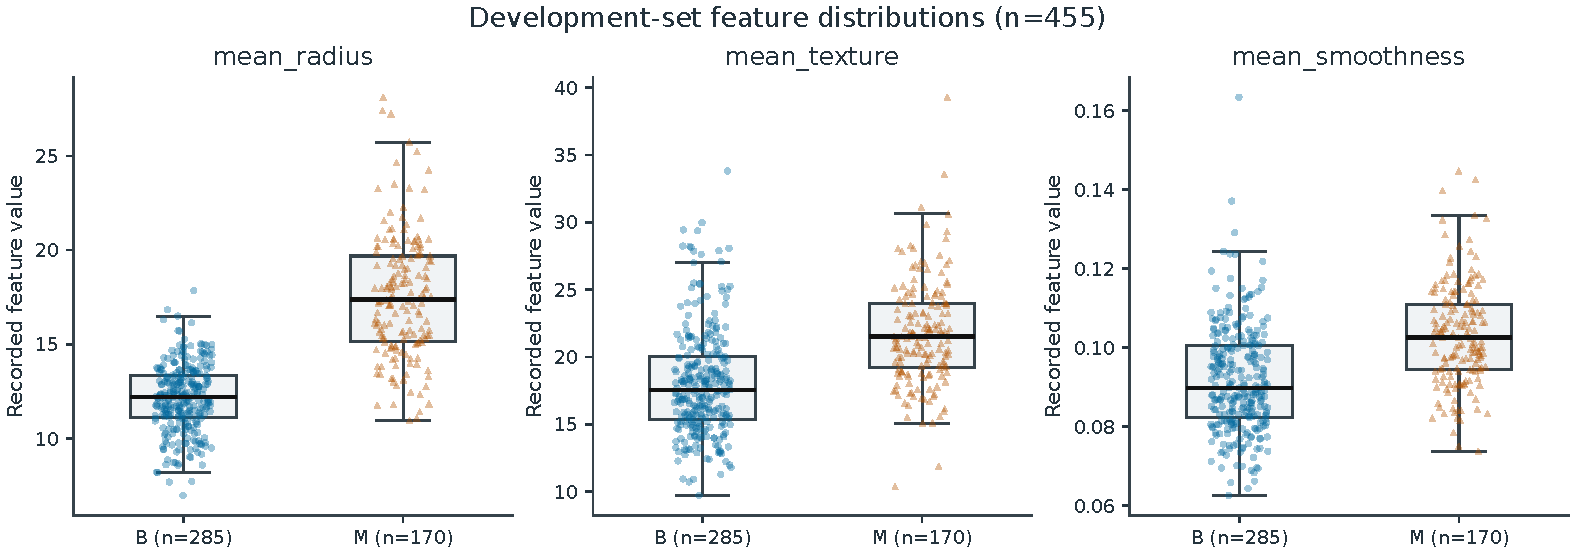
\includegraphics[width=0.94\linewidth,height=0.48\textheight,keepaspectratio]{figures/feature_distributions.pdf}
\caption{开发集三项预设特征的组间分布。图中显示实际观测的离散和重叠，不因其影响分类表现而删除合理极端值。}\label{fig:descriptive}
\end{figure}

\begin{figure}[htbp]\centering
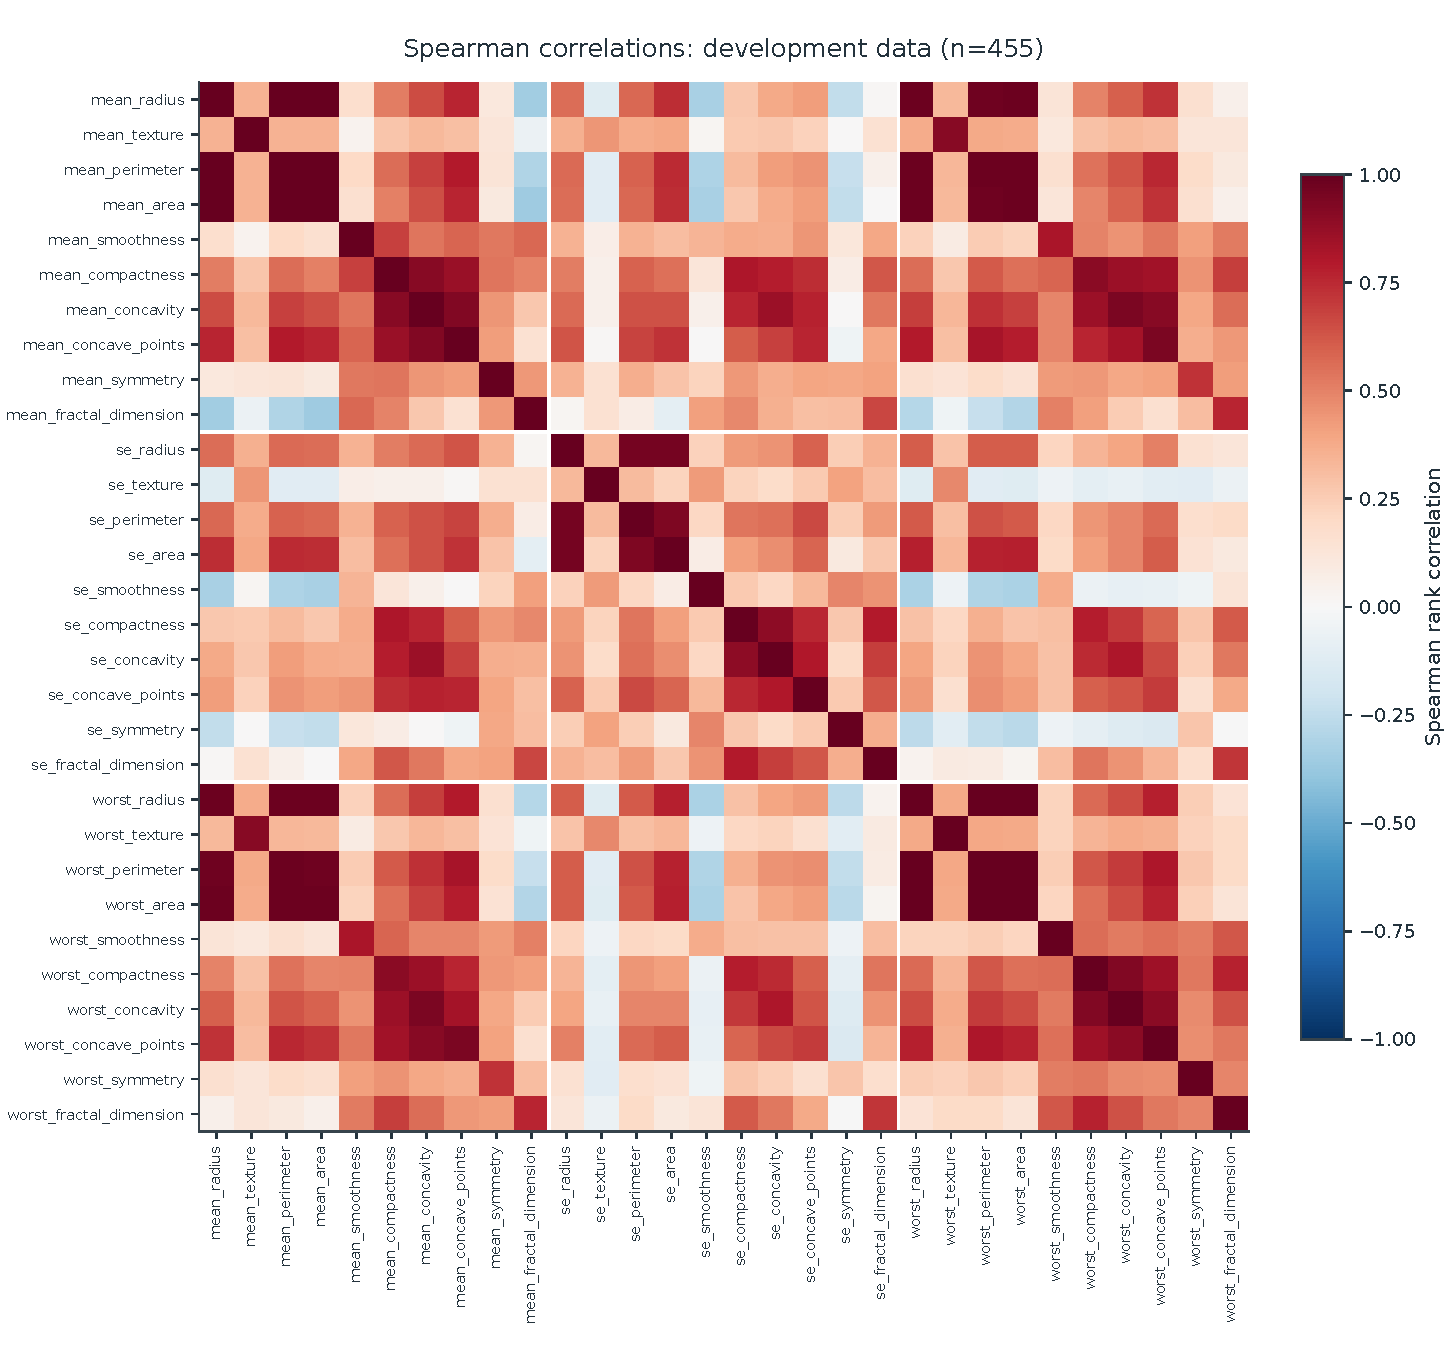
\includegraphics[width=0.94\linewidth,height=0.48\textheight,keepaspectratio]{figures/spearman_heatmap.pdf}
\caption{开发集 30 个特征的 Spearman 相关结构。颜色表示相关系数；该图为探索性描述，不对所有相关系数进行显著性筛选。}\label{fig:correlation}
\end{figure}

\FloatBarrier

\subsection{开发集比较与最终测试}
下表将开发集 CV 与最终测试结果分开呈现。主比较始终是 LR30、LR10、LR5；RF30 的作用是提供另一模型族的参照，DUMMY 用于显示类别比例基线。
\begin{center}
\small
\setlength{\tabcolsep}{5pt}
\renewcommand{\arraystretch}{1.25}
\begin{tabular}{lrrrr}
\toprule
模型 & 特征数 & 开发集 CV AUC & 测试 AUC & 测试 AUC 95\% 区间 \tabularnewline
\midrule
DUMMY & 0 & 0.5000 $\pm$ 0.0000 & 0.5000 & [0.5000, 0.5000] \tabularnewline
LR30 & 30 & 0.9958 $\pm$ 0.0052 & 0.9960 & [0.9871, 1.0000] \tabularnewline
LR10 & 10 & 0.9851 $\pm$ 0.0134 & 0.9974 & [0.9911, 1.0000] \tabularnewline
LR5 & 5 & 0.9850 $\pm$ 0.0126 & 0.9957 & [0.9868, 1.0000] \tabularnewline
RF30 & 30 & 0.9870 $\pm$ 0.0076 & 0.9940 & [0.9838, 1.0000] \tabularnewline
\bottomrule
\end{tabular}
\end{center}
{\footnotesize CV 为共用分层五折上的均值与标准差，标准差不是置信区间。DUMMY 不利用特征与标签的关联。}

三个逻辑回归模型的开发集平均 CV AUC 分别为 \LRFullCVAUC{}、\LRTenCVAUC{}、\LRFiveCVAUC{}；最终测试 AUC 分别为 \LRFullAUC{}、\LRTenAUC{}、\LRFiveAUC{}。本次 LR10 的测试 AUC 略高于 LR30，但其开发集 CV 均值较低；两套评价上的排序并不完全一致，不能因此在测试后把展示默认模型改为 LR10 或宣称它普遍优于完整模型。
\begin{figure}[htbp]\centering
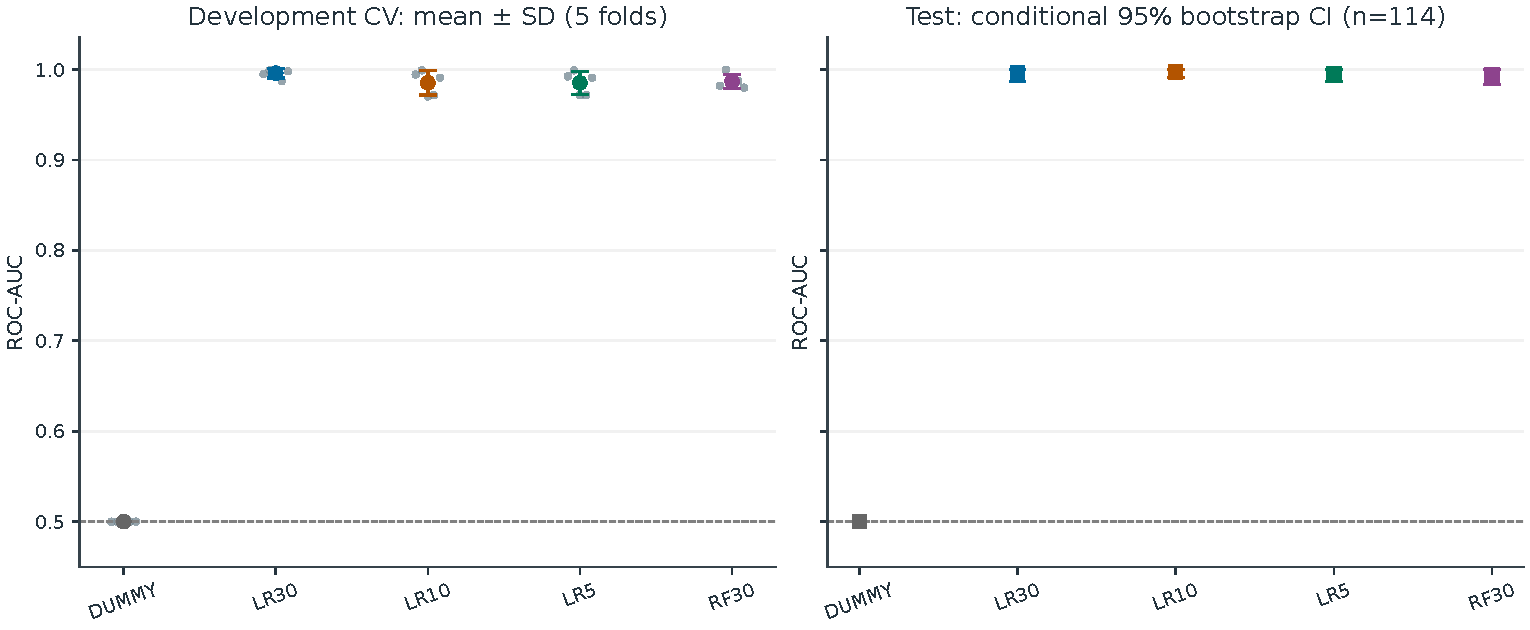
\includegraphics[width=0.94\linewidth,height=0.48\textheight,keepaspectratio]{figures/model_performance.pdf}
\caption{预设模型的开发集交叉验证与最终测试表现。两部分使用的数据不同；CV 标准差与测试 bootstrap 区间分别解释。}\label{fig:performance}
\end{figure}

测试集中，LR30、LR10、LR5 的恶性召回率分别为 \LRFullSensitivity{}、\LRTenSensitivity{}、\LRFiveSensitivity{}。相应漏判为 \LRFullFN{}、\LRTenFN{}、\LRFiveFN{} 条，误判恶性为 \LRFullFP{}、\LRTenFP{}、\LRFiveFP{} 条。相近的 AUC 不意味着固定阈值下错误计数完全相同，因而需要同时查看排序评价与分类结果。
\begin{center}
\small
\setlength{\tabcolsep}{5pt}
\renewcommand{\arraystretch}{1.25}
\begin{tabular}{lrrrrr}
\toprule
模型 & 灵敏度 & 特异度 & 精确率 & F1 & 准确率 \tabularnewline
\midrule
DUMMY & 0.000 & 1.000 & 未定义 & 0.000 & 0.632 \tabularnewline
LR30 & 0.929 & 0.986 & 0.975 & 0.951 & 0.965 \tabularnewline
LR10 & 0.905 & 0.986 & 0.974 & 0.938 & 0.956 \tabularnewline
LR5 & 0.929 & 0.986 & 0.975 & 0.951 & 0.965 \tabularnewline
RF30 & 0.905 & 1.000 & 1.000 & 0.950 & 0.965 \tabularnewline
\bottomrule
\end{tabular}
\end{center}
{\footnotesize 阈值均为 0.5。无阳性预测时精确率未定义，表中明确标出；F1 依实际评价实现报告。}

\begin{center}
\small
\setlength{\tabcolsep}{5pt}
\renewcommand{\arraystretch}{1.25}
\begin{tabular}{lrrrr}
\toprule
模型 & TN：正确良性 & FP：误判恶性 & FN：漏判恶性 & TP：正确恶性 \tabularnewline
\midrule
DUMMY & 72 & 0 & 42 & 0 \tabularnewline
LR30 & 71 & 1 & 3 & 39 \tabularnewline
LR10 & 71 & 1 & 4 & 38 \tabularnewline
LR5 & 71 & 1 & 3 & 39 \tabularnewline
RF30 & 72 & 0 & 4 & 38 \tabularnewline
\bottomrule
\end{tabular}
\end{center}
{\footnotesize 全部计数来自同一最终测试集。准确率较高不意味着没有漏判。}

\begin{figure}[htbp]\centering
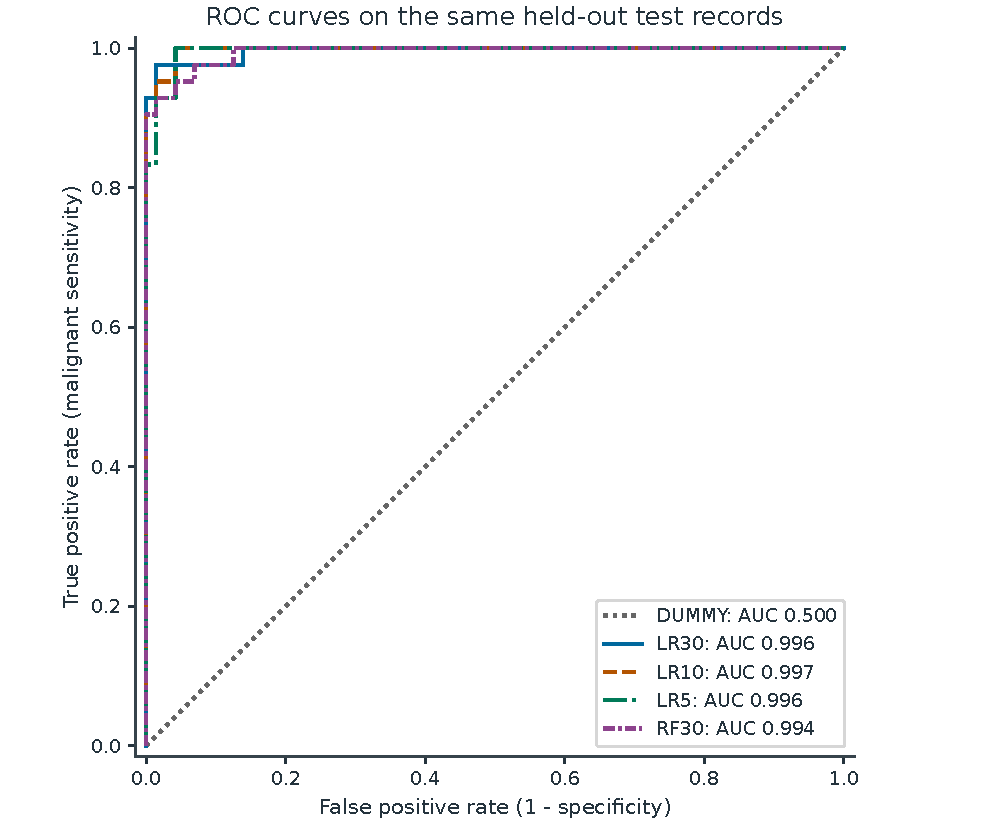
\includegraphics[width=0.94\linewidth,height=0.48\textheight,keepaspectratio]{figures/test_roc.pdf}
\caption{最终测试集 ROC 曲线。所有模型在同一批测试样本上评价，使用恶性类别的连续预测分数。}\label{fig:roc}
\end{figure}

\FloatBarrier

\subsection{减量差值与不确定性}
\begin{center}
\small
\setlength{\tabcolsep}{5pt}
\renewcommand{\arraystretch}{1.25}
\begin{tabular}{lrr}
\toprule
测试集 AUC 差值 & 点估计 & 成对 bootstrap 95\% 区间 \tabularnewline
\midrule
LR5-LR30 & -0.0003 & [-0.0103, 0.0093] \tabularnewline
LR10-LR30 & 0.0013 & [-0.0063, 0.0103] \tabularnewline
\bottomrule
\end{tabular}
\end{center}
{\footnotesize 1,000 次按真实类别分层的成对重采样。差值为减量模型减去 LR30；负值表示减量模型的 AUC 较低。}

LR5-LR30 的差值为 -0.0003，95\% 区间为 [-0.0103, 0.0093]；区间包含 0，无法凭本次结果认定差异方向已稳定确定。
LR10-LR30 的差值为 0.0013，95\% 区间为 [-0.0063, 0.0103]；区间包含 0，无法凭本次结果认定差异方向已稳定确定。
这些差值只涉及同一测试集上的预设比较，不能通过是否跨零推导临床非劣效或安全性。由于测试集规模有限，即使只改变少数恶性样本的排序或判断，也可能改变评价结果。
\begin{figure}[htbp]\centering
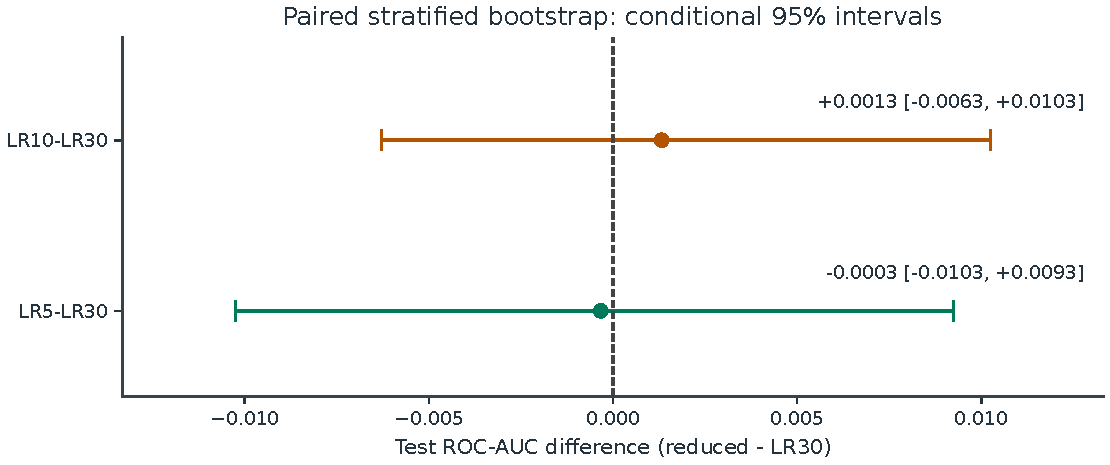
\includegraphics[width=0.94\linewidth,height=0.48\textheight,keepaspectratio]{figures/auc_differences.pdf}
\caption{减量模型相对 LR30 的测试 AUC 差值及成对 bootstrap 不确定性。所有模型在每次重采样中使用相同样本索引。}\label{fig:bootstrap}
\end{figure}

\FloatBarrier

\subsection{入选特征、系数与错误解释}
\begin{center}
\small
\setlength{\tabcolsep}{5pt}
\renewcommand{\arraystretch}{1.25}
\begin{tabular}{l>{\raggedright\arraybackslash}p{0.79\linewidth}}
\toprule
模型 & 完整开发集最终拟合时保留的特征 \tabularnewline
\midrule
LR10 & \texttt{mean\_radius}, \texttt{mean\_perimeter}, \texttt{mean\_area}, \texttt{mean\_concavity}, \texttt{mean\_concave\_points}, \texttt{worst\_radius}, \texttt{worst\_perimeter}, \texttt{worst\_area}, \texttt{worst\_concavity}, \texttt{worst\_concave\_points} \tabularnewline
LR5 & \texttt{mean\_perimeter}, \texttt{mean\_concave\_points}, \texttt{worst\_radius}, \texttt{worst\_perimeter}, \texttt{worst\_concave\_points} \tabularnewline
\bottomrule
\end{tabular}
\end{center}
{\footnotesize 名单来自最终拟合，不是先在全数据筛选得到。不同交叉验证折可能产生不同名单。}

图~\ref{fig:selection} 展示开发集各折入选频次，横向附录图~\ref{fig:coefficients} 展示最终逻辑回归系数。相关变量可能替代彼此进入较小特征集；入选频次高表示对当前训练划分较稳定，并不证明它是独立病因。最终系数受标准化、正则化及其他入模变量影响，不能把不同模型中系数变化直接理解为变量真实效应变化。
\begin{figure}[htbp]\centering
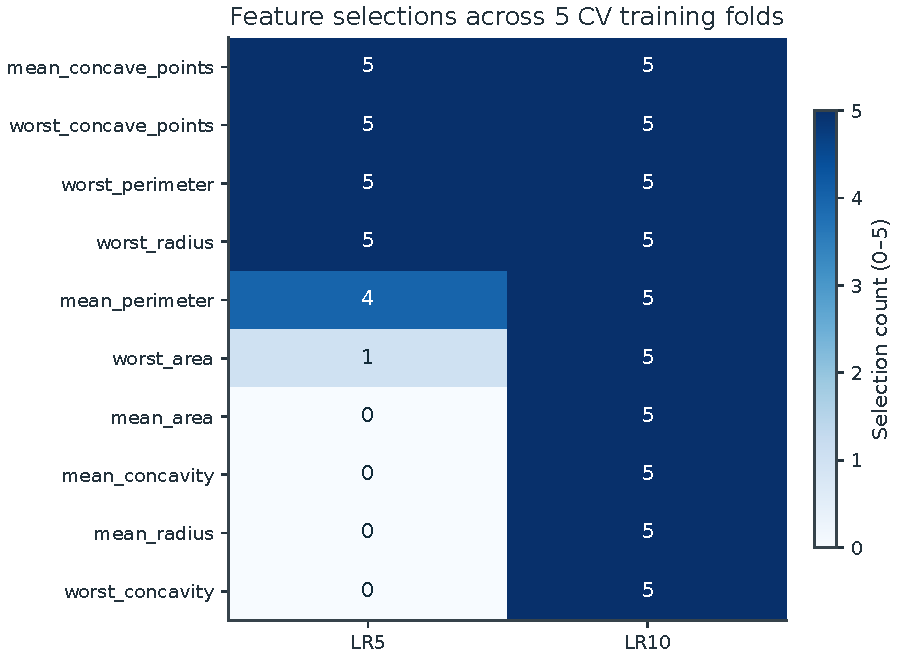
\includegraphics[width=0.94\linewidth,height=0.48\textheight,keepaspectratio]{figures/selection_frequency.pdf}
\caption{五折训练中减量模型的特征入选频次，范围为 0--5。该频次只描述本次划分下的选择稳定性，不是真实入选概率。}\label{fig:selection}
\end{figure}

依据保存的逐条测试预测，LR30 与 LR5 分别误判 4、4 条记录，误判样本集合的交集为 0 条。在同一批 114 条测试记录中，两模型对 8 条给出不同类别预测（7.0\%）。本次两模型的 FN 与 FP 汇总计数相同，但不能据此认为它们错误的样本相同。这些数值是既定误判分析下的探索性描述，不保证组合模型能够改善表现，也不据此更改默认模型。

误判记录保存在项目内部预测输出中，可通过样本标识回查。错判分析用于说明模型错误及特征重叠，不为个体作诊断解释；仅凭这份特征表无法确定某次漏判对应的临床病理原因。网页展示汇总错误计数，避免将个案展示包装成实际诊疗建议。
\FloatBarrier

\section{讨论与局限}
本项目在相同划分、模型设置和评价规则下比较三种输入数量，回答的是当前数据集上的模型简化问题。主要结果应综合 AUC 差值、区间、灵敏度、错误计数以及筛选稳定性判断；不能仅选最高的测试分数作为结论。若少量变量模型表现接近，它说明在此验证条件下部分信息可能冗余，并不意味着已找到最优特征组合或证明临床等效。

首先，WDBC 是经典公开数据，分类标签和特征来自特定既有收集过程。当前记录缺少支持跨机构、年代、年龄或族群验证的信息；本作业没有外部验证，也不能完成这些亚组的公平性结论。其次，\TestN{} 条测试记录中的恶性样本为 \TestM{} 条，评价仍有较大样本不确定性；当前 bootstrap 没有覆盖训练过程变异。第三，单变量筛选可能保留相关变量，也可能错过依赖变量组合的信号；固定参数控制了比较范围，但不代表每个模型的最优性能。第四，逻辑回归系数和特征入选是预测关联，不构成病因判断。第五，概率分数未进行独立校准与临床效用验证，阈值 0.5 仅是统一比较规则。

最后，特征来自同类细针穿刺图像，减少列数不等于减少侵入性检查、检查费用或患者负担。后续研究可以在独立来源数据上考察稳定性和校准，并预先规定真正有意义的简化标准；这些工作不属于本次课程结果。

\section{课程实现、可复现性与成果展示}
本项目用 pandas 完成无表头 CSV 的读取、类型和质量核查；用 NumPy 与 SciPy 组织数组计算、分布检验和重采样；用 scikit-learn 的管道完成训练内预处理、筛选、模型拟合及评价；用 Matplotlib/Seaborn 生成图表。类与方法、函数、字典、循环及文件路径管理贯穿分析。统计分析、模型评价与网页展示分别对应课程的不同评分环节。

报告由 \texttt{scripts/build\_report.py} 读取 \texttt{outputs/summary.json}，生成汇总数字、表格和图引用；逐条预测文件 \texttt{outputs/predictions/test\_predictions.csv} 用于计算两模型的错误重合与预测不一致情况。脚本核对该文件的行数、类别计数及混淆计数，并在 \texttt{public\_report/provenance.json} 中记录两个结果源的 SHA-256，避免手工抄录造成漂移。原始数据校验值、软件版本、随机种子、参数、划分和预测结果保存在项目中。重建报告本身不会训练模型；应先执行分析入口生成真实输出，再重建和编译。现有结果与新环境是否一致，需要实际复跑核验。

\begin{itemize}
\item 个人主页：\HomepageURL。
\item 项目展示页：\ProjectURL。
\item 代码仓库：\RepositoryURL。
\end{itemize}
网页以同一批分析输出为依据，提供 5/10/30 特征方案切换，联动显示特征名单、测试 AUC、恶性召回率及混淆计数。切换只改变预先计算结果的展示，不重新训练，也不据测试表现临时改选模型。仓库首页与本地 HTML 文件不能自动替代公开可访问的个人主页和项目页面；发布后还需在未登录状态下核验链接与下载。

\section{结论}
本作业完成了 WDBC 数据的规范读取、质量检查、开发集统计分析、训练内特征选择及预设模型的独立测试评价。LR30、LR10、LR5 的测试 AUC 为 \LRFullAUC{}、\LRTenAUC{}、\LRFiveAUC{}；特征减量的价值需结合相应不确定性、错误计数和可解释性共同判断。结论限于本公开数据和当前验证设计，不宣称临床等效、降低检查费用或可以直接用于诊断。

\section*{AI 辅助与软件说明}
本项目使用 Codex 辅助设计实现、整理结果及起草报告，并参考 Scientific Agent Skills 的科学写作与方法核查流程\cite{agentskills}. AI 不是作者；署名者需要理解并核对代码、实际输出、文字、引用及页面内容，确认最终提交。所有结果数字来自实际分析输出，AI 辅助不替代实验执行，也不替代对引用和结论的人工核验。

\bibliographystyle{unsrtnat}
\bibliography{references}
\FloatBarrier
\appendix
\clearpage\begin{landscape}\thispagestyle{plain}
\begin{figure}[p]\centering
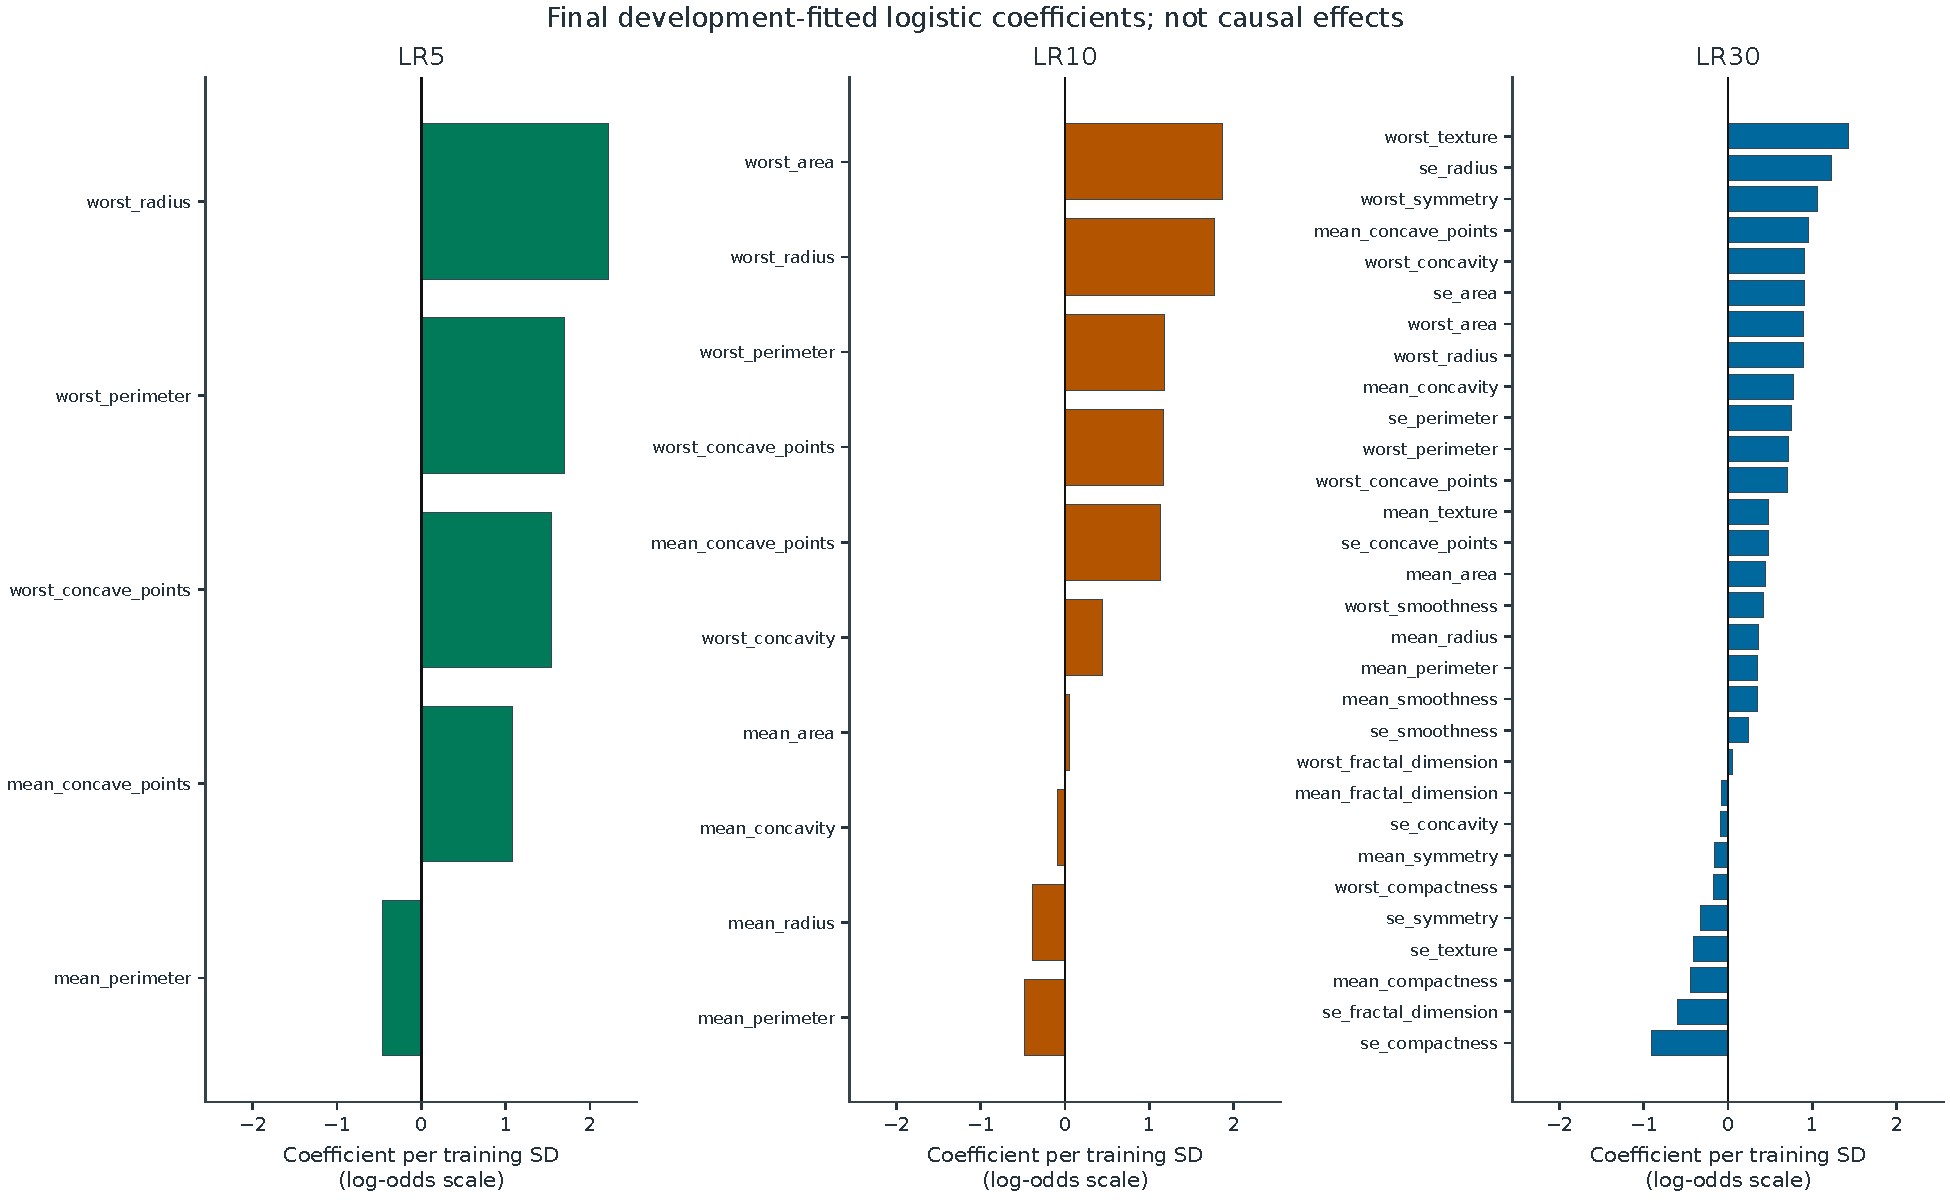
\includegraphics[width=0.98\linewidth,height=0.88\textwidth,keepaspectratio]{figures/logistic_coefficients.pdf}
\caption{在完整开发集拟合的逻辑回归模型的标准化系数。系数反映模型内的条件预测关联，受正则化和特征相关性影响。}\label{fig:coefficients}
\end{figure}\end{landscape}\clearpage

\section{质量核查与软件版本}
\begin{center}
\small
\setlength{\tabcolsep}{5pt}
\renewcommand{\arraystretch}{1.25}
\begin{tabular}{p{0.57\linewidth}p{0.3\linewidth}}
\toprule
核查项（与输出字段名一致） & 结果 \tabularnewline
\midrule
rows & 569 \tabularnewline
input\_features & 30 \tabularnewline
missing\_feature\_values & 0 \tabularnewline
nonfinite\_feature\_values & 0 \tabularnewline
duplicate\_ids & 0 \tabularnewline
duplicate\_feature\_rows & 0 \tabularnewline
duplicate\_full\_rows & 0 \tabularnewline
unknown\_labels & 0 \tabularnewline
excluded\_rows & 0 \tabularnewline
id\_excluded\_from\_predictors & True \tabularnewline
\bottomrule
\end{tabular}
\end{center}

\begin{center}
\small
\setlength{\tabcolsep}{5pt}
\renewcommand{\arraystretch}{1.25}
\begin{tabular}{ll}
\toprule
软件 & 实际版本 \tabularnewline
\midrule
numpy & 2.5.4 \tabularnewline
pandas & 3.1.0 \tabularnewline
scipy & 1.18.1 \tabularnewline
scikit-learn & 1.9.1 \tabularnewline
statsmodels & 0.15.0 \tabularnewline
matplotlib & 3.11.2 \tabularnewline
seaborn & 0.13.2 \tabularnewline
joblib & 1.6.0 \tabularnewline
pillow & 13.0.0 \tabularnewline
\bottomrule
\end{tabular}
\end{center}

\noindent 原始 CSV 的 SHA-256：\par
{\footnotesize\ttfamily\seqsplit{d606af411f3e5be8a317a5a8b652b425aaf0ff38ca683d5327ffff94c3695f4a}}

\section{提交前核对}
\begin{enumerate}
\item 核对作者署名、个人主页和项目页面；未发布地址不能标为已完成。
\item 对照输出表检查样本数、标签方向、AUC、错误计数和区间。
\item 确认能够解释 Pipeline、特征选择和测试集用途。
\item 检查 PDF 图表、参考文献和链接；公开页面以未登录访问为准。
\item 明确保存真实代码、参数和重跑说明，由署名者完成最终审阅。
\end{enumerate}
\end{document}
